% !TEX root = twibop2.tex
\chapter{Probability in the Microcosm}
\begin{epigraphs}
\qitem{To date quantum theory led us to a deeper comprehension: it established a closer relation between statistics and the fundamentals of physics. This is an event in the history of human thought, whose significance is beyond science itself.} {M. Born}

\vspace{10pt}

\qitem{Quantum mechanics allowed us to postulate the existence of primary probabilities in the laws of nature.}  {W. Pauli}
\end{epigraphs}


\section{Spontaneous Micro-processes}

Classical physics proceeded from that randomness only reveals itself in
large collections, for instance, in ensembles of molecules, in appreciable
volumes of gas. However, classical physics did not see randomness in
the behaviour of individual molecules. The investigations resulting in the
appearance and development of \redem{quantum physics} showed that this
viewpoint was invalid. It turned out that randomness is seen both in
ensembles of molecules and in the behaviour of individual molecules.
This is demonstrated by \redem{spontaneous} microprocesses.

\txthead{Neutron decay.} A typical example of a spontaneous microprocess is
the decay of a free neutron. Usually, neutrons are in a bound state.
Together with protons, they are the ``bricks'' from which atomic nuclei
are built. However, neutrons can also be observed outside nuclei, in the
free state. For instance, free neutrons appear when uranium nuclei split.
It turns out that a free neutron can \redem{randomly, without any external influence}, transform into three particles: a proton, an electron, and an
antineutrino (more accurately, an electron antineutrino). This
transformation is called neutron decay, and it is commonly written
down as:
\begin{equation*}%
n \to p + e^{-} + \bar{\nu}_{e},
\end{equation*}
where $n$ is a neutron, $p$ is a proton, $e^{-}$ an electron, and $\bar{\nu}_{e}$ is an antineutrino. Note that the term ``decay'' is not entirely suitable here because it conveys the idea that a neutron consists of a proton, electron, and antineutrino. In reality, all three particles are born at the moment the neutron annihilates, and it is no use looking for them ``inside'' the neutron.

The very fact of spontaneous neutron decay is \redem{random}, but there is
also a dialectic necessity here as well. In order to reveal it, we should
consider a large number of neutrons. Suppose there are $N_{0}$ neutrons in a volume at moment $t = 0$, where $N_{0} \gg 1$. Let us measure the number of neutrons in the volume at different moments $t$, the result being a function $N (t)$ whose plot has a certain shape (\figr{decay-fn}). The resultant
function is
\begin{equation}%
N(t) = N_{0} \, \exp \, ( - \,a \,t),
\label{eq-5.1}
\end{equation}
where $a$ is a constant and is commonly given as $1/\tau$, measurements
show that $\tau = \SI{d3}{\second}$.

\begin{figure}[!ht]
\centering
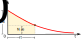
\includegraphics[width=0.75\textwidth]{figures/decay.pdf}
\sidecaption{The number of neutrons decaying as a function of time.\label{decay-fn}}
\end{figure}

The value $\tau$ is called the neutron's \redem{lifetime}. It is called this
conventionally not because it is the true lifetime of a neutron, but
because it is the time needed for the number of intact (un-decayed)
neutrons to decrease e times. Whence from \eqref{eq-5.1} we have 
\begin{equation*}
\frac{N\,(t)}{N_{0}} = \exp \left( -\frac{t}{\tau} \right) = \frac{1}{e}.
\end{equation*}
The true lifetime of a neutron may vary considerably from
$\tau$ in both directions. It is in principle impossible to predict when
a neutron will decay. We can only consider the \redem{probability} that
a neutron will live a while until it decays. When the number of neutrons
is large, the ratio $N\, (t) / N_{0}$ is the probability that a neutron will survive for a time $t$. It follows from \eqref{eq-5.1} that this probability is $\exp (-t / \tau)$.

I would like to draw your attention to an interesting detail. When we
discuss the probability that a neutron will survive for a time $t$, we do
not suppose that this interval is measured from the moment of the
neutron's birth. It is not essential how long a neutron has lived by $t = 0$.
The probability that it will survive a further time $t$ is always equal to
$\exp  (-t / \tau)$. It can be said that neutrons ``do not get old''. This means that there is no meaning in looking for the cause of the neutron's decay
within its ``internal mechanism''.

It is interesting that \eqref{eq-5.1}, which expresses a certain necessity, is
nothing but a direct consequence of the fact that the decays occur
independently and randomly. Since the decay is a random process, the
decrease in the number of neutrons (in other words, the number of
decays) $\Delta N$ during an interval of time from $t$ to $t + \Delta t$ is proportional to the number of neutrons $N (t)$ at that instant and the lapse of time $\Delta t$, i.e. $ \Delta N = - a \, N \, (t) \, \Delta t$. Let us rewrite this equality as   $ \Delta N / \Delta t  = - a \, N \, (t)$. In the
limit as $ \Delta \, t \to 0$, we obtain a differential equation known as the \redem{equation of exponential decay}:
\begin{equation}%
\frac{dN}{dt} = a \, N \, (t).
\label{eq-5.2}
\end{equation}
The function \eqref{eq-5.1} is the solution of this equation given the initial condition $N (0) = N_{0}$.

In conclusion, let me remark that if a neutron is not free but is bound
with protons and other neutrons in an atomic nucleus, it loses its ability
to decay. However, it regains this ability in some cases. The
phenomenon of beta decay is then observed (we shall discuss it below).

\txthead{The instability of elementary particles.} The neutron is not at all the only elementary particle that turns spontaneously into other particles.
Most elementary particles possess this property, which might be called
\redem{instability}. There are only several particles that are stable: the photon, the neutrino, the electron, and the proton.

The instabilities of different particles teach us additional things of
randomness. For instance, let us take the particle called the sigma-plus-hyperon $\Sigma^{+}$. It has a positive electric charge equal in its absolute value to the charge of electron, and has a mass 2328 times that of an electron. Like the neutron, this particle decays spontaneously. Its lifetime (this term is understood in the same way as it was for a neutron) is $0.8 \times \SI{d-10}{\second}$. Unlike the neutron, the hyperon may decay in two ways: 
\begin{equation*}%
\text{either} \,\,  \Sigma^{+} \to p + \pi^{0}  \qor  \Sigma^{+} \to n + \pi^{+}.
\end{equation*}
($\pi^{0}$ and $\pi^{+}$ are neutral and positively charged pions, respectively).  Approximately 50 per cent of the hyperons decay in one way, and the others decay in the other way. We cannot unambiguously predict either when the hyperon decays or how.

\txthead{The instability of atomic nuclei (radioactivity).} Each element may
have several types of atomic nuclei. They contain the same number of
protons (the atomic number determining the position of the element in
the periodic table), but the number of neutrons in them differs; these
different nuclei are called \redem{isotopes}. Most isotopes of an element are
\redem{unstable}. The unstable isotopes of an element transform spontaneously into isotopes of other elements simultaneously emitting particles. This phenomenon is called \redem{radioactivity}. It was first discovered by the French physicist Antoine Henry Becquerel (1852-1908) in 1896. The term ``radioactivity'' was introduced by Pierre Curie (1859-1906) and Marie Sklodowska-Curie (1867-1934) who investigated the phenomenon and won the Nobel Prize for physics (with A.H. Becquerel) in 1903.

Investigations showed that the lifetime of unstable isotopes is
essentially different for different isotopes and follow different decay
routes (different types of radioactivity). The lifetime of an isotope may
be measured in milliseconds, or it may be years or centuries. There are
isotopes with lifetimes of over \num{d8} years. The study of long-lived
unstable isotopes in nature have allowed scientists to determine the age
of rocks.

Let us discuss different types of radioactivity. Let us use $Z$ to denote
the number of protons in a nucleus (the atomic number of an element)
and use $A$ to denote the sum of the number of protons and neutrons in
the nucleus (the mass number). One type of radioactivity is called \redem{alpha decay}. During the process, the initial nucleus $(Z, A)$ decays into an
alpha-particle (a helium nucleus, which consists of two protons and two
neutrons) and a nucleus with two less protons $(Z - 2)$ and a mass
number four units smaller $(A - 4)$:
\begin{equation*}%
X(Z, A) \to \alpha \, (2, 4) + Y(Z - 2, A - 4).
\end{equation*}
Another type of radioactivity is \redem{beta decay}. During this process, one of the neutrons in the initial atomic nucleus turns into a proton, an
electron, and an antineutrino, like a free neutron does. The proton stays
within the new nucleus while the electron and the antineutrino escape.
The scheme of beta decay can be presented as:
\begin{equation*}%
X (Z, A) \to Y(Z + 1, A) + e^{-} + \bar{\nu}_{e}.
\end{equation*}
\redem{Proton radioactivity} is also possible:
\begin{equation*}%
X(Z, A) \to p + Y(Z - 1, A - 1).
\end{equation*}
Let me draw your attention to the \redem{spontaneous fission} of atomic
nuclei. The initial nucleus disintegrates spontaneously into two
``fragments'' (two new nuclei), approximately equal in mass, and several
free neutrinos are formed in the process.

A chain of consecutive spontaneous transformations is shown in
\figr{spon-fission}. The neptunium isotope \ce{^{237}Np} $(Z = 93, \,\, A = 237)$ finally turns into the stable isotope of bismuth \ce{^{20}Bi} $(Z = 83, \,\,A = 209)$. The chain consists of ``links'' corresponding to alpha decays (the blue arrows in the figure) and beta decays (the red arrows). The lifetime (in the probabilistic sense) is indicated by each arrow. These chains are called \redem{radioactive
families} (or series).

\begin{figure}[!ht]
\centering
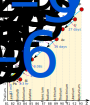
\includegraphics[width=0.8\textwidth]{figures/spont-fission.pdf}
\sidecaption{The number of neutrons decaying as a function of time.\label{spon-fission}}
\end{figure}

\txthead{Induced and spontaneous transitions in an atom.} The reader will
know that the energy of an atom can only have a set of discrete values
that are specific to each atom. These allowed states of the atom are
called \redem{energy levels}. When we excite atoms by irradiating them, they
jump from low energy levels to higher ones. The excited atoms return to
the lower levels by emitting light. These jumps are called \redem{quantum
transitions}.


A quantum transition may be either \redem{induced} (stimulated) or
\redem{spontaneous}. Transitions due to the excitation of an atom are always
induced. The reverse transitions may be both induced and spontaneous.

For simplicity's sake, let us only consider two atomic energy levels:
energies $E_{1}$ and $E_{2}$ (\figr{emission}). The transition $E_{1} \to E_{2}$ is an induced and occurs when an atom absorbs a photon with energy $\varepsilon_{12} = E_{2} - E_{1}$ The atom may return to level $E_{1}$ either spontaneously or by being induced to. A photon with energy $\varepsilon_{12}$ is emitted in the process. The spontaneous transition $E_{2} \to E_{1}$ is a random event. The induced transition $E_{2} \to E_{1}$ is caused when a photon passes near the atom. The energy of the photon should be equal to $\varepsilon_{12}$. The figure shows each of these three processes: 

\begin{enumerate}[label=(\alph*),noitemsep,nolistsep]
\item the absorption of a photon with energy $\varepsilon_{12}$ by the atom (atom transition  $E_{1} \to E_{2}$ ), 
\item the spontaneous emission of a photon with energy $\varepsilon_{12}$ by the atom (atom transition $E_{2} \to E_{1}$) , and
\item the induced emission of a photon possessing energy $\varepsilon_{12}$ by the atom while it interacts with the stimulating primary photon also possessing energy $\varepsilon_{12}$ (atom transition $E_{2} \to E_{1}$).
\end{enumerate}

\begin{figure}[!ht]
\centering
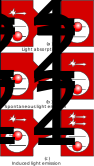
\includegraphics[width=0.7\textwidth]{figures/emission.pdf}
\sidecaption{Induced and spontaneous emissions in a two level quantum system.\label{emission}}
\end{figure}


It should be noted that the photon emitted during an induced
transition, as it were, copies every property of the primary photon that
caused the atom transition. For instance, it moves in the same direction
as the primary photon.


\txthead{How does a laser generate radiation?} Many books on science for the general reader cover lasers and explain the induced emission of photons
as being due to simultaneous emission by a large number of specially
selected atoms or molecules (they are called \redem{active centres}). The photons resulting from induced radiation move in the same direction, thus
forming laser radiation (laser is the abbreviation for light amplification
by stimulated emission of radiation).

The explanation of how a laser generates is commonly given as
follows. First, the active centres are excited, for instance, by an intense
flash of light. It is necessary that the number of active centres in the higher
energy level should be greater than those in the lower one. Then
photons begin to appear with an energy equal to the difference between
the energies of the higher and lower levels of the active centres, and the
active centres radiate by induced emission more often than the reverse
process (the process of photon absorption) occurs. This is easy to see if
we take into account that each primary photon can cause with equal
probability the transition of an active centre both upwards (the process
of light absorption) and downwards (induced emission). Therefore,
everything depends on whether the number of active centres is greater
in the higher or in the lower level. If there are more centres in the higher
level, more downward transitions will occur i.e. induced emission
prevails. The result is an intense beam of laser photons.

\begin{figure}[!ht]
\centering
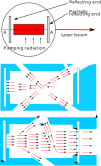
\includegraphics[width=0.75\textwidth]{figures/laser.pdf}
\sidecaption{ A schematic explanation of how does the laser emission works.
\label{laser}}
\end{figure}

Everything is correct in this explanation. However, most writers
ignore the appearance of the primary photons which induce emission of
the new photons and trigger the process of laser generation. The protons
appear due to the \redem{spontaneous} transition of active centres from the
higher level to the lower one. Because they are so important for lasers,
we should not forget the \redem{primacy} (and fundamentality) of the
spontaneous emission processes. We could stop discussing lasers at this
point. However, a reader might want to ask some questions.

\begin{dialogue}

\rdr ``You said that the induced photon copies every property of
the primary photon, in particular, its direction of motion.''

\athr ``Quite right.''

\rdr ``But spontaneous transitions yield photons moving in
random directions. Therefore, the induced photons should also move
in random directions. A photon that has appeared spontaneously,
passing by a number of excited active centres, will induce an
avalanche of photons in the direction it is moving in. The second
spontaneous photon will cause an avalanche of induced photons in
another direction, and so on. Now how come a laser beam has
a single direction?''

\athr ``You have made an essential point. Suppose $AA$ is the beam
direction (\figr{laser}). The active medium of a laser is formed into a cylinder with its long axis in the $AA$ direction. Two mirrors (end plates) are placed at right angles to $AA$, one mirror being partially
silvered: it lets the emission out. Some photons will be randomly born
in the $AA$ direction (or close enough to it), and then will pass the
active substance along a relatively long path, which is increased
because it might be reflected many times from the mirrors at both
ends. By interacting with induced active centres, these photons, sooner
or later, will cause a powerful flux of induced photons to appear, and
these form the laser beam. Photons randomly born in other directions
and their associated induced photons will only travel a short distance
along the active substance and will very soon be `out of play'. This
can be seen clearly in the figure.''

``Let me note that the mirrors which set the direction of the laser
beam constitute the \redem{resonator} of the laser.''

\rdr ``So the laser radiation appears from noise (spontaneous
radiation) owing to the \redem{selectivity} of amplification, i.e. because the
amplification occurs mainly in a certain direction.''

\athr ``Exactly. Once again we encounter the \redem{selection of
information from noise}. The ordered (coherent) laser radiation is, as it
were, selected from noise by the mirrors (end plates) of the resonator.
The \redem{amplification} of selection occurs owing to induced emission: when the secondary photon copies the properties of the primary one.''


\end{dialogue}

\section{From Uncertainty Relations the Wave Function}

As we discussed spontaneous micro-processes, we found that the random
in the microcosm reveals itself even in the behaviour of an individual
body. This brings us close to a discussion of the \redem{primacy} and
\redem{fundamentality} of the notion of probability in quantum mechanics. We shall start with the \redem{uncertainty principle} suggested in 1927 by the German physicist Werner Heisenberg (1901-1976).

\txthead{Uncertainty relations.} A micro-body moving according to the laws of quantum mechanics does not have, strictly speaking, a trajectory of
motion. This is because a micro-body does not have both a momentum
and a set of coordinates \redem{simultaneously}. Suppose a micro-body has
a certain $x$-component of its momentum. It turns out that the
$x$-coordinate of the micro-body in this state does not have any certain
value. The other extreme case corresponds to the state of a micro-body
in which, vice versa, its $x$-coordinate has a certain value while the
$x$-component of its momentum does not. There are an infinite number
of intermediate cases when both the $x$-coordinate of the body and the
$x$-component of its momentum are not certain, although they take
values within certain intervals.

Suppose $\Delta \, x$ is the interval within which the $x$-coordinate values lie;
let us call $\Delta \, x$ the \redem{uncertainty} of the $x$-coordinate. Let us consider the uncertainty of the $x$-component of the momentum $\Delta \, p_{x}$ in a similar way. Heisenberg showed that the uncertainties $\Delta \, x$ and $\Delta \, p_{x}$ are related as:
\begin{equation}%
\Delta \, x \, \Delta \, p_{x} \approx \hbar,
\label{eq-5.3}
\end{equation}
where $\hbar = 1.05 \times \SI{d-34}{\joule\second}$ is Planck's constant. Similar relations can be written down for other components of the coordinates and the momentum of the microbody: $\Delta \, y \, \Delta \, p_{y} \approx \hbar$ and $\Delta \, z \, \Delta \, p_{z} \approx \hbar$.

These are Heisenberg's famous \redem{uncertainty relations}. We shall limit
ourselves to a discussion of the \redem{coordinate-momentum} uncertainty
relations. However, there are similar relations for some other pairs of
variables, for instance, for \redem{energy} and \redem{time}, and \redem{angle} and the \redem{moment of momentum}. Heisenberg wrote that we cannot interpret the processes on the atomic scale as we might a large-scale process. However, if we use common notions, their applicability is limited by the uncertainty relations.

When we discuss the uncertainty relations, we shall only use \eqref{eq-5.3}. Do not, however, think that this relation outlaws accurate measurements of the momentum or coordinates of a micro-body. It only states that a micro-body cannot simultaneously have both accurately defined coordinates and an accurately defined momentum. For instance, if we try to measure the $x$-coordinate of a micro-body more accurately (in other words, to decrease $\Delta \, x$), we will cause its momentum's $x$-component to become more uncertain. In the limit when the
$x$-coordinate of the micro-body has a certain value (the micro-body is
accurately localized), the uncertainty of the $x$-component of its
momentum becomes very large. And vice versa, establishing the
$x$-component of the micro-body's momentum more accurately
unavoidably causes its x-coordinate to become more uncertain.

Let us consider a plane in which the $x$-coordinate of a body is plotted
along one axis (the $x$-axis) and its momentum's $x$-component is plotted
along the other axis (the $p_{x}$-axis) (\figr{unc}). If the body obeyed the laws of classical mechanics, its any state would be a point in the plane. However, the state of a micro-body corresponds to a rectangle with area $\hbar$. Other types of state are also possible. They correspond to rectangles of various shapes. Some of them are presented in the figure.

\begin{marginfigure}[-2cm]
\centering
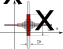
\includegraphics[width=1.\textwidth]{figures/unc.pdf}
\caption{ States of a micro-body.\label{unc}}
\end{marginfigure}

\txthead{Uncertainty relations and the wave properties of a micro-body}. In
1924, the French physicist Louis de Broglie (b.~1892) hypothesized that
a microbody possesses the properties of both a \redem{particle} and a \redem{wave}. Its particle characteristics (energy $\varepsilon$ and momentum $p$), de Broglie postulated, are related to its wave characteristics (frequency $\omega$ and wavelength $\lambda$) thus:
\begin{equation}%
\varepsilon = \hbar \, \omega \qand p = 2 \pi \, \hbar / \lambda.
\label{eq-5.4}
\end{equation}
This hypothesis seemed absurd to many physicists. They could not
understand what a particle's wavelength might be.

In 1927, a striking result was obtained during experiments in which
an electron beam was sent through thin metal plates. After leaving the
plate the electrons spread out in a \redem{diffraction} pattern (\figr{diffraction1}). \redem{Electron diffraction} by a crystalline lattice became an experimental fact, and yet diffraction and interference are wave properties. Therefore, the experiments on electron diffraction were unanimously accepted as proof of the wave properties of the electron. The nature of the electron waves remained as puzzling as before, but nobody doubted their existence.

\begin{figure}[!ht]
\centering
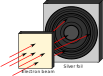
\includegraphics[width=0.75\textwidth]{figures/diffraction-01.pdf}
\sidecaption{ Electron diffraction experiment proved the wave properties of the electrons.\label{diffraction1}}
\end{figure}

We shall return to the waves below. Let us use de Broglie's hypothesis
to explain the uncertainty relations. Suppose that a strictly parallel
electron beam with a momentum $p$ passes through a plate with a very
marrow slit whose width in the $x$-direction is $d$ (the $x$-axis is at right
angles to the beam) (\figr{diffraction2}). 

The electrons are diffracted when they pass through the slit. According to classical wave theory, the angle through which the electrons are diffracted to the first diffraction maximum is $\theta \approx \lambda / d$. If we use $\lambda$ as the wave characteristic of the electron and use the second relation in \eqref{eq-5.4}, we can write $\theta$ as $\theta \approx \hbar /p \, d$. However, what does the angle $\theta$ mean in terms of particles? In fact what happens is that when the electron passes through the slit, it acquires a momentum $\Delta \, p_{x}$ in the $x$-direction. Clearly,  $\Delta \, p_{x} \approx p \, \theta$ . Since $ \theta \approx \hbar /p \, d$, we obtain  $\Delta \, p_{x} \, d \approx \hbar$. If $d$ is thought of as the uncertainty  $\Delta \, {x}$  of the $x$-coordinate while the electron passes through the slit, we obtain the uncertainty relation \eqref{eq-5.3}.



\begin{marginfigure}%[-4cm]
\centering
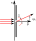
\includegraphics[width=0.9\textwidth]{figures/diffraction-02.pdf}
\caption{ Electron diffraction experiment as understood by the uncertainty of the momentum and direction.\label{diffraction2}}
\end{marginfigure}


\txthead{The wave function.} Suppose a micro-body is in a state such that the $x$-component of its momentum has a value $p_{0}$. We know that the value of the $x$-coordinate of the micro-body in this state is very uncertain. In other words, the micro-body may be found at any place on the $x$-axis.

Does this mean that we can say nothing about the $x$-coordinate of the
micro-body? No, it does not. It turns out that. we can establish the
probability that the micro-body's $x$-coordinate takes a value from $x$ to
$x + \Delta \, x$. This probability can be written as $\abs{\Psi_{p_{0}}  (x)}^{2} \, \Delta \, x$.

We see that the probability density needed to find the micro-body at
a point $x$ is the square of the function $\Psi_{p_{0}}  (x)$. This function is
commonly called the \redem{wave function}. The reader should not understand the term ``wave'' literally. The point is that in the 1930s the researchers looking at the microcosm got so carried away by wave concepts (due to the experiments on electron diffraction) that they spoke of ``wave 	mechanics'' rather than ``quantum mechanics''.

Thus, the state of a micro-body such that the $x$-component of its
momentum possesses a value $p_{0}$ and given that the $x$-coordinate does not have any certain value is described by the wave function $\Psi_{p_{0}} (x)$ whose squared absolute value is the probability density of the
micro-body to be found at point $x$. I want to emphasize that the results
of measuring a micro-body's coordinate in state $\Psi_{p_{0}} (x)$ prove to be \redem{random} each time. A value of the coordinate is realized with the
probability density $\abs{\Psi_{p_{0}}  (x)}^{2}$.

I have only selected one state of the micro-body without dealing with,
for instance, the states where both the momentum and coordinate are
uncertain. Besides, I limited the discussion to the coordinate and
momentum without dealing with other variables, for instance, energy or
the moment of momentum. I believe that this is sufficient to see the
main point: any state of a micro-body is described by a function defining
the probability (or the probability density) of some characteristics of the
micro-body. Thereby it is clear that quantum mechanics of even one
micro-body is a \redem{probabilistic} theory.

\txthead{The electron in the atom.} The electrons in atoms may occur in
different states. A change in the electron's state may, for instance, be
related to the atom's transition from one energy level to another. Let us
put down possible states of an electron in an atom by means of wave
functions $\Psi_{j}(x, y, z)$, where $j$ is a set of some numbers characterizing a state and $(x, y, z)$ are coordinates of the electron. Given what we said above, we can conclude that $\abs{\Psi_{j}(x, y, z)}^{2}$ is the density of probability that we can find an electron in state $j$ at point $(x, y, z)$. Now imagine an ``object'' whose density is proportional to $\abs{\Psi_{j}(x, y, z)}^{2}$ at various points of space. We can imagine a cloud with the density varying from point to point. The density inside the cloud is the greatest. While the point approaches the surface of the cloud, the density falls to zero, and thus the cloud has some \redem{shape} (although without a distinct bounding surface).

\begin{figure}[!ht]
\centering
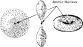
\includegraphics[width=0.8\textwidth]{figures/orbitals.pdf}
\sidecaption{ Electron clouds in an atom.\label{orbitals}}
\end{figure}

This ``cloud'' is the probabilistic ``image'' of an electron in an atom.
Several ``electron clouds'' are shown in \figr{orbitals} for the electron's several states in an atom.

\section{Interference and Summing Probability Amplitudes}

After reading this section, we shall see that the probabilities in the
microcosm obey the laws we have not dealt with above. It is noteworthy
that these laws allow us to make a rather unexpected conclusion,
namely that interference and diffraction are possible in principle even in
the absence of waves. They may be an effect of \redem{specific rules for the
summation of probabilities.}

\txthead{The puzzling behaviour of a microbody in an interferometer.} Without discussing the technical details, let us consider an experiment in which particles pass through an interferometer containing two close slits and
then are detected on a special screen (\figr{double-slit}). 

\begin{figure}[!ht]
\centering
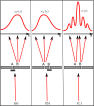
\includegraphics[width=0.8\textwidth]{figures/interference.pdf}
\sidecaption{The two slit experiment.\label{double-slit}}
\end{figure}
Let us consider the $x$-coordinate of the particles. In order to deal with a \redem{probability} rather than a \redem{probability density}, suppose that the $x$-axis on the screen is separated into small identical intervals, so that when we speak of the probability that a particle arrives at a point $x$ we mean the probability of arriving at the appropriate part of the axis around point $x$.

Suppose slit $A$ is closed while slit $B$ is open. After a large enough
number of particles have been detected on the screen, we obtain
a distribution defined by the function $w_{B} (x)$ (\figr{double-slit}~\drkgry{(a)}). This function is the probability that a particle passing through slit $B$ (when slit $A$ is closed) will arrive at point $x$. Given our remarks in the preceding section, we have
\begin{equation}%
w_{B} \, (x) = \abs{\Psi_{B} (x)}^{2},
\label{eq-5.5}
\end{equation}
where $\Psi_{B}(x)$ is the wave function for the particle passing through slit $B$. I should remark that recently the term ``wave function'' is being more
often substituted by a better term, ``probability amplitude'' (or ``probability density amplitude''). Therefore, the probabilistic nature of
the particle's state is emphasized in this way. We shall now use the term
\redem{probability amplitude} and not wave function. Thus,  $\Psi_{B}(x)$ is the probability amplitude that a particle will arrive at point $x$ after passing
through slit $B$ (when slit $A$ is closed).

Now suppose that slit $B$ is closed while slit $A$ is open. If this is the case, the screen (Fig. 5.9b) will show the distribution $w_{A} (x)$:
\begin{equation}%
w_{A} (x) = \abs{\Psi_{A}  (x)}^{2},
\label{eq-5.6}
\end{equation}
where $\Psi_{A}(x)$ is the probability amplitude of a particle arriving at point
$x$ after passing through slit $A$ (when slit $B$ is closed).

And finally, let us open both slits. It would be natural to believe that
if it passes through one of the slits, a particle ``does not feel'' the other
slit. It can be said that it is ``indifferent'' as to whether the other slit is
open or closed. And in this case the distribution on the screen should be
the sum of distributions \eqref{eq-5.5} and \eqref{eq-5.6}, which, by the way, corresponds to the rule of \redem{probability summation}: 
\begin{equation}%
w_{AB} \, (x) = w_{A} \, (x) + w_{B} \, (x) =  \abs{\Psi_{A} \, (x)}^{2} +  \abs{\Psi_{B} \, (x)}^{2}.
\label{eq-5.7}
\end{equation}
In reality, the screen yields a typical \redem{interference} distribution
 (\figr{double-slit}~\drkgry{(c)}).  rather than distribution \eqref{eq-5.7}. It turns out that when it passes through one slit the particle somehow ``feels'' the other slit. Or, perhaps more incomprehensible, the particle somehow manages to pass through both slits at the same time. How does it actually pass the
interferometer?

\txthead{``Spying'' destroys the interference pattern.} Let us try and ``spy'' on
how the particle behaves when both slits are open. The ``spying'' would
seem to be possible in principle. For instance, we might place a source
of light near each slit and detect the photons reflected by the particles
near each slit. Such experiments have in fact been carried out. They
showed that the particle passes through only one slit, and at the same
time it turned out that the distribution on the screen was described by
\eqref{eq-5.7}. This means that ``spying'' helps establish the details of the particle's passing through the interferometer, but the interference distribution is destroyed.

We have thus a curious situation. If the light is turned off (no
``spying''), there is interference, but the mechanism by which the particle
passes through the interferometer cannot be uncovered. If the light is on,
the mechanism can be ascertained, but the interference distribution is destroyed.


When should we sum up probabilities and when probability amplitudes? Let me start to explain the amazing results described above. A particle has two options (two alternatives): to pass through either slit $A$ or slit $B$. If the light is off, these alternatives are \redem{indistinguishable}. They become \redem{distinguishable} if the light is on, and therefore, ``spying'' or, in terms of science, observation is possible.

One of the basic conclusions of quantum mechanics is that 
\begin{mybox}{}
if alternatives are distinguishable, the respective probabilities are to be
summed up; but if the alternatives are indistinguishable, probability
amplitudes rather than probabilities are summed up. 
\end{mybox}
Therefore, when the light is on, the probabilities should be summed up, but when the light is off, the probability amplitudes should be summed up. In the former
case, we arrive at distribution \eqref{eq-5.7}, and in the latter case, we obtain the distribution
\begin{equation}%
w_{x} \, (x) =  \abs{\Psi_{A} \, (x) +  \Psi_{B} \, (x)}^{2}.
\label{eq-5.8}
\end{equation}
This is an interference distribution. It can be shown that
\begin{equation}%
 \abs{\Psi_{A} +  \Psi_{B}}^{2} =  \abs{\Psi_{A}}^{2} +  \abs{\Psi_{B} \, (x)}^{2} + \left[ \frac{\Psi_{A}}{\Psi_{B}} \,\abs{\Psi_{B}}^{2} + \frac{\Psi_{B}}{\Psi_{A}}\, \abs{\Psi_{A}}^{2} \right].
\label{eq-5.9}
\end{equation}
The expression in the square brackets is ``responsible'' for the
interference nature of the distribution $w(x)$. In classical physics, the
problem of distinguishable (indistinguishable) events does not exist since
classical events are always distinguishable. In the microcosm, the
situation is qualitatively different. Here we encounter the possibility of
complete \redem{indistinguishability} of some random events. This possibility arises because of the fundamental \redem{identity} of all particles of the same type. An electron is like any other to a far greater extent than the proverbial two peas in a pod. Naturally, electrons may be in different
states, which allows us to distinguish between them. However, any
electron (as a physical particle) is indistinguishable from any other
electron. Here we are dealing with absolute identity. In the last analysis,
it allows for indistinguishable alternatives. 

We see that interference should not be limited to wave concepts. The
interference in microphenomena is not necessarily related to waves, it
may be a consequence of probabilistic laws, or more accurately,
a consequence of the fact that we should sum up probability amplitudes
rather than probabilities for indistinguishable events.

\txthead{Quantum-mechanical superposition.} Consider
\begin{equation}%
 \Psi_{A} \, (x) +  \Psi_{B} \, (x)= \Psi \, (x).
\label{eq-5.10}
\end{equation}
The function $\Psi \, (x) $ in quantum mechanics is on an equal footing with
functions $ \Psi_{A} \, (x)$ and $ \Psi_{B} \, (x)$ and like them it defines a state, or rather the probability amplitude for a random event. In this case, $ \Psi_{A} \, (x)$ is the amplitude of the probability that a particle arrives at point $x$ after passing through the interferometer with two open slits. This amplitude is said to be the \redem{superposition} of the amplitudes $ \Psi_{A} \, (x)$ and $ \Psi_{B} \, (x)$.


It is impossible to imagine such a superposition in a demonstrative
way. Otherwise, we should quite seriously have to believe that the
particle passes simultaneously through both slits ($A$ and $B$). Any attempt
to reveal the details of this event \redem{destroys the superposition}. It is
destroyed each time either in favour of $ \Psi_{A}$ (the particle passed through slit $A$) or in favour of $ \Psi_{B} $ (the particle passed through slit $B$). Here we encounter one more manifestation of the random. We have
noted above that the arrival of the particle at a point on the screen is
a random event, and probabilities \eqref{eq-5.7} and \eqref{eq-5.8} characterize these random events. It turns out that the ``selection'' of a slit by a particle is also random. The particle passes through slit $A$ with a probability proportional to  $ \abs{\Psi_{A}}^{2}$ and passes through slit $B$ with a probability proportional to $ \abs{\Psi_{B}}^{2}$.

\txthead{A wave or the sum of probability amplitudes?} The wave concept
explains the appearance of interference patterns best. However, the wave
concept cannot explain the other phenomenon, the destruction of the
interference pattern by ``spying''. In other words, a wave can explain the
\redem{appearance} of quantum-mechanical superposition, but it cannot explain the \redem{destruction} of the superposition in the process of observation.

Once convinced of this and the futility of the attempts to make ``de
Broglie's waves'' material, physicists admitted that these ``waves'' have
nothing in common with really existing waves. This gave rise to a very
expressive term of \redem{probability waves}. Gradually, the term ``wave
mechanics'' has been substituted everywhere by the term ``quantum
mechanics'' while the term ``wave function'' has become more often
replaced by the term ``probability amplitude''.

Therefore, we should explain both the interference and diffraction of
particles in terms of the necessity of summing up probability amplitudes
instead of probabilities rather than in terms of enigmatic waves when
the considered alternatives are indistinguishable. The probabilistic
approach completely explains both the appearance and destruction of
quantum-mechanical superposition.

In conclusion, let us consider a situation which illustrates the limited
nature of the wave approach. We shall discuss the diffusion of very slow
neutrons passing through a crystal.

\txthead{Diffusion of neutrons in a crystal.} A beam of neutrons with energies of only \SI{0.1}{\eV} is passed through a crystal. The neutrons diffused by the crystal's nuclei are registered by a system of detectors (counters) along the $x$-axis (\figr{neutron-diff}). The crystal contains $N$ nuclei, therefore, there are $N$ alternatives. Each alternative corresponds to the diffusion of a neutron by a nucleus. Let us use $ \Psi_{j} \, (x)$ to denote the probability amplitude that a neutron will arrive at the detector at point $x$ after diffusing past the $j$-th nucleus.
\begin{marginfigure}%[!ht]
\centering
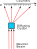
\includegraphics[width=0.9\textwidth]{figures/neutron-diff.pdf}
\caption{Diffraction of neutrons through a crystal.\label{neutron-diff}}
\end{marginfigure}

It is interesting that the diffusion of a neutron by a nucleus may occur
in two ways. In one case the neutron's \redem{spin is inverted} while there is no such inversion in the other case. Let me explain. A neutron can be
represented as a rotating top. The top may rotate in either one direction
or the other, the neutron's spin being said to be either upwards or
downwards, respectively. The crystal's nuclei are also reminiscent of
rotating tops, i.e. they each have spin directions. When a neutron (top)
collides with a nucleus, it mayor may not change the direction of its
	rotation. In the former case, the neutron's spin remains unchanged while
in the latter it is reversed. If a diffused neutron changes the direction of
its rotation, the direction of rotation of the nucleus at which the act of
diffusion occurred should somehow change as well. Therefore, if
diffusion occurs with one neutron's spin inversion, we are dealing with
a \redem{distinguishable} alternative. We can state that diffusion occurred
precisely at the nucleus which changed the direction of its rotation. If
diffusion occurs without spin inversion, it is in principle impossible to
indicate which nucleus diffused the neutron; here we deal with an
\redem{indistinguishable} alternative.


Suppose $\varphi$ is the probability amplitude that a neutron will diffuse
with spin inversion while $\chi$ is the probability amplitude without
inversion. Let us use $\Phi  (x)$ to denote the probability amplitude that
a neutron with inverted spin will arrive at point $x$, and $X  (x)$ the same for a neutron with noninverted spin. The distribution of diffused neutrons
detected by the counters can be presented as:
\begin{equation}%
w_{x} \, (x) =  \abs{\varphi }^{2}\, \abs{\Phi \, (x) }^{2}  + \abs{\chi}^{2} \, \abs{X \, (x)}^{2}.
\label{eq-5.11}
\end{equation}
Naturally, the alternatives corresponding to different types of neutron
diffusion are distinguishable; therefore, probability $w(x)$ consists of two
terms (two probabilities are summed up). In turn, each term is the
product of two probabilities.


Now let us express $ \abs{\Phi \, (x) }^{2}$ and $ \abs{X \, (x) }^{2}$ in terms of amplitudes  $\Psi_{j} \, (x)$. If a neutron is diffused with spin inversion, the alternatives are distinguishable; therefore, the \redem{probabilities are summed up}, and hence
\begin{equation}%
\abs{\Phi \, (x) }^{2} = \sum_{j=1}^{N} \abs{\Psi_{j} \, (x) }^{2}.
\label{eq-5.12}
\end{equation}
\begin{marginfigure}%[!ht]
\centering
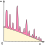
\includegraphics[width=\textwidth]{figures/neutron-dist.pdf}
\caption{Distribution of diffraction of neutrons through a crystal.
\label{neutron-dist}}
\end{marginfigure}
If the spin of a diffused neutron has not been inverted, the alternatives
are indistinguishable; therefore the probability amplitudes are to be
summed up (amplitude superposition occurs) and hence
\begin{equation}%
|X \, (x) |^{2} = \left| \sum_{j=1}^{N} |\Psi_{j} \, (x) |^{2} \right|.
\label{eq-5.13}
\end{equation}
Substituting \eqref{eq-5.12} and \eqref{eq-5.13} into \eqref{eq-5.11}, we obtain:
\begin{equation}%
w(x) = \left[  |\varphi |^{2} \,\,  \sum_{j=1}^{N} |\Psi_{j} \, (x) |^{2} \right] + \left[  |\chi |^{2} \,\,  \sum_{j=1}^{N} |\Psi_{j} \, (x) |^{2} \right] . 
\label{eq-5.14}
\end{equation}
The distribution of diffused neutrons $w(x)$ in experiment is shown in
\figr{neutron-dist}. It consists of a smoothly varying ``background'' and a set of interference maxima. The ``background'' is defined in \eqref{eq-5.14}) by the term in the first square brackets while the interference maxima give the term in the second square brackets.

Using wave concepts, we have to assume that a neutron has the wave
properties while diffusing without spin inversion (the interference pattern
appears). The same neutron does not show any wave properties in
diffusion with spin inversion (the interference pattern does not appear).
It is evident that this assumption is quite unnatural.

\section{Probability and Causality }

\begin{dialogue}

\rdr ``I think there is too much randomness in the microcosm.
A neutron suddenly turns into three new particles at random, without
any external influence. An atom may be at rest for many years and
then suddenly, for no apparent reason, decays and turns into an atom
of another chemical element. An electron randomly passes through
a slit in the interferometer and quite as randomly arrives at a point
on the screen. Doesn't it mean that, in fact, there is no \redem{causality} in the phenomena of the microcosm?''

\athr ``No, it doesn't. The phenomena of the microcosm show
very explicitly the \redem{dialectical unity of the random and the necessary}. Neutrons decay in a random manner, but their quantity varies in time
according to a certain law. An electron randomly arrives at a point on
the screen, but the distribution of arrivals of many electrons is
necessary. There are no grounds for doubting existence of causality in
the microcosm. We should bear in mind that causality in the
microcosm reveals itself unlike that in the macrocosm. In quantum
mechanics, potential possibilities to realize events or, in other words,
the \redem{probabilities} of these events are only causally related, rather than individual realized events themselves. The probability amplitude (wave function) obeys a definite equation of motion. Knowing the
probability amplitude at the initial moment and using this equation (it
is called \redem{Schr\"odinger's equation}), we can find the probability amplitude at an arbitrary moment in time.''

\rdr ``It is not clear why a neutron should suddenly decay.
Maybe, the particles in question are, in fact, more complex systems
whose physical nature is not yet known'?''

\athr ``We touched on this in our first talk. I said that the search
for \redem{hidden parameters}, which would explain why, for instance,
a neutron decays, eventually, at a given moment in time proved to be
unsuccessful. But I would like to show what is behind the posed
question. Asking it, you proceed from that probability in the
microcosm is \redem{not objective} but related with our lack of knowing \redem{some details}. I think that both the examples from the microcosm and many of the examples from our macrocosm we cited convinced you that probability can be both subjective (related to a lack of knowledge) and objective. This is essential. It is only when probability is objective that we can say that probabilistic regularities are primary, or fundamental.''

\rdr ``Please explain this idea.''

\athr ``If probability were reduced to a lack of information, it
could be reduced in principle to dynamic relations supposing unambiguous
prediction. This would mean that the probabilistic laws would
conceal the dynamic ones. In this case it could be possible to assume
that, in the last analysis, everything is strictly interrelated in the
Nature.''

\rdr ``But doesn't any event, any phenomenon have a cause in the
long run?''

\athr ``You're right to mention causality. However, why do you
believe that the existence of objective probability means the absence
of causality?''

\rdr ``Objective probability suggests objective randomness. And
this randomness reveals itself without any cause, because it is related
to chance.''

\athr ``I throw a die, and, say, the four comes up. You throw
a die, and the three comes up. Are these events objectively random or
not? What do you think?''

\rdr ``Each event has definite causes. The occurrence of an event
depends, over a long stretch, on the position of the die in your hand,
the wave of hand, the push, the air resistance, the distance from the
hand to the floor, etc.''

\athr ``Right. And nonetheless, the events are not objectively
random ones. Throwing a die, you are not interested in the way
I threw mine. We are not interested in how a die is thrown at all, do
not try to control and direct our actions. Therefore, the occurrence of
the four on my die and the three on yours are objectively random
events. The occurrence of the three is not related to the occurrence of
the four just before it.''

\rdr ``I don't quite understand.''

\athr ``I can give you another example. Suppose the events are
telephoned taxi orders. Each order conceals a chain of causes.
However, the arriving orders are objectively random events for the
taxi-depot dispatcher. And this is not because he does not know the
chain of causes but because of an objective circumstance, namely the
lack of connection between the actions of the people making orders
for taxi. The events are considered, as it were, in two different planes.
In one, they are objectively random, while in the other each of them
has definite causes. As you see, objective probability agrees with
causality.''

\rdr ``Your example is from practice. And what about
microphenomena? Let us once again take the example with neutron
decay. Suppose this event is objectively random in a `plane'. But in
what plane should we look for the causes for the neutron decay?''

\athr ``Neutron decay is indeed objectively random. We cannot
control the lifetime of a given neutron in principle because of deep
reasons and not a lack of knowledge about some details. There is no
internal ``clock'' in a neutron. As was noted above, neutrons ``do not
get old''. This can be seen in that a neutron may live for some time
irrespective of how long it has already lived by the moment we start
counting time. Because it is objectively random, neutron decay is not
a causeless event. I want to note that when we speak of the
\redem{spontaneous} behaviour of a particle, we are being inaccurate. Strictly speaking, only a hundred per cent \redem{isolated} particle can behave \redem{spontaneously}. And here we come close to a fundamental point which we haven't discussed yet.''

``The point is that a particle is \redem{not isolated}, it interacts with the
world around it. It is in essence dependent on the conditions of each
concrete situation. The term `interaction' should be understood here
in a wider meaning than it is understood when considering usual
(force) interactions.''

\rdr ``New puzzles of quantum mechanics.''

\athr ``I do not mean any puzzles. At a certain level of investigation of physical phenomena, isolation is lost in principle. For instance, the distinct boundary between the field and the matter is erased. The mutual transformations of particles become apparent. The idea of the \redem{unity of the world and the universal interrelation of the phenomena in it} acquires a special meaning on the level of the microcosm.''

\rdr ``How can we imagine in a demonstrative way that a decaying neutron is not isolated?''

\athr ``A \redem{vacuum} in quantum mechanics is not a void but a space in which particles are randomly born and annihilated. The neutron interacts with them.''
\end{dialogue}
%%% Local Variables:
%%% mode: latex
%%% TeX-engine: xetex
%%% TeX-master: "twibop2"
%%% End:
